
\documentclass[aspectratio=169,11pt]{beamer}
% customize block aesthetics
\definecolor{customblue}{rgb}{0.13,0.28,0.59}
\setbeamercolor{block title}{bg=customblue, fg=white}
\setbeamercolor{block body}{bg=customblue!10}
\setbeamertemplate{blocks}[rounded]
\usepackage{array,color,graphicx,comment,tikz}
\usepackage{bibentry,amsmath,verbatim}
\bibliographystyle{abbrv}
\setbeamertemplate{bibliography entry title}{}
\setbeamertemplate{bibliography entry location}{}
\setbeamertemplate{bibliography entry note}{}
\setbeamercolor{bibliography entry author}{fg=black}
\setbeamercolor{bibliography entry title}{fg=gray}
%\usetikzlibrary{calc,patterns,decorations.pathmorphing,decorations.markings}
\input talk_defs.tex
%\input formatting.tex

\mode<presentation>
{
\usetheme{default}
}

\setbeamertemplate{navigation symbols}{}
\usecolortheme[rgb={0.13,0.28,0.59}]{structure}
\setbeamertemplate{itemize subitem}{--}
\newcommand\footlineon{
\setbeamertemplate{footline} {
\begin{beamercolorbox}[ht=2.5ex,dp=1.125ex,leftskip=.8cm,rightskip=.6cm]{structure}
%\footnotesize \insertsection
\hfill
{\insertframenumber}
\end{beamercolorbox}
\vskip 0.45cm
}
}
\footlineon

\AtBeginSection[] 
{ 
	\begin{frame}<beamer> 
		\frametitle{Outline} 
		\tableofcontents[currentsection,currentsubsection] 
	\end{frame} 
}
\usepackage{listings}
%%% Custom listing format
\definecolor{seagreen}{rgb}{0.18, 0.55, 0.34}
\definecolor{mediumviolet-red}{rgb}{0.78, 0.08, 0.52}
\definecolor{khaki}{rgb}{0.94, 0.9, 0.55}
\definecolor{background-gray}{gray}{0.95}
\setbeamertemplate{footline}{
  \hfill 
  \usebeamerfont{page number in head/foot}
  \usebeamercolor[fg]{page number in head/foot}
  \small 
  \insertframenumber \hspace*{2ex} \vspace*{2ex} 
}

\lstdefinelanguage{mypython}
{
keywords=[1]{from, import, as, assert, not, print, nonneg, PSD, qcp, pos, axis,
             for, in, bool},
keywordstyle=[1]{\color{mediumviolet-red}},
keywords=[2]{surecr, torch, cp, lo, pl, cvxpy, dsp, Variable, LocalVariable,
        sqrt, exp, saddle_inner, saddle_max, saddle_min, SaddlePointProblem, MinimizeMaximize,
        numpy, np, Problem, Minimize, Maximize, is_dsp, solve, inner,
        convex_variables, concave_variables, affine_variables, sum, mean, multiply,
        triu, astype, reshape,
        arange, range, norm1, norm2, norm_inf, abs, square, saddle_quad_form, norm,
        sum_values, sum_squares, inv_pos, huber, diff, log, log_sum_exp, Parameter,
        append, ones, diag, np, power, ppf, quad_over_lin, cholesky,
        diagonal, outer, array, linalg, inv, log_det, quad_form, status, hstack},
keywordstyle=[2]{\color{seagreen}},
upquote=true,
showstringspaces=false,
basicstyle=\ttfamily\small,
columns=fullflexible,
keepspaces=true,
emph={True,False,def,return,float,class,match,switch,len},
emphstyle={\color{seagreen}},
backgroundcolor = \color{background-gray},
belowskip=1em,
aboveskip=1em,
morecomment=[l]{\#}
}
%% begin presentation
\title{
A Prescient Analysis of Optimal Energy Storage
}

\author{
\textbf{Giray Ogut}\inst{1} \and 
Bennet Meyers\inst{2} \and
David Chassin\inst{2} \and
Kirsten Perry\inst{3} \and \\
Stephen Boyd\inst{1} \and
}

\institute{
\inst{1} Stanford University \\
\inst{2} SLAC National Accelerator Laboratory \\
\inst{3} National Renewable Energy Laboratory
}

\date{\small REGROW Quarterly Report, 9/9/2024}

\begin{document}

\begin{frame}
\titlepage
\end{frame}

\begin{frame}{Single-node model}
\BIT
\item \textbf{setting:}  \\
\hspace{12mm} $-$ node in Central Valley, CA part of WECC grid\\
\hspace{12mm} $-$ realistic load and renewable data for 2018 (hourly resolution)\\
\item \textbf{prescient:} \\
\hspace{12mm} $-$ load and renewable for the entire year known beforehand\\
\hspace{12mm} $-$ storage, generation and shortfall variables\\
\hspace{12mm} $-$ single optimization problem\\
\hspace{12mm} $-$ minimize fossil generation and shortfall\\
\hspace{12mm} $-$ subject to physical constraints\\
\item \textbf{motivation:} \\
\hspace{12mm} $-$ upper bound on performance\\
\hspace{12mm} $-$ simplification, sanity checks, pedagogy\\
\EIT
\end{frame}

\begin{frame}{Dataset}
	
\begin{figure}
\centering
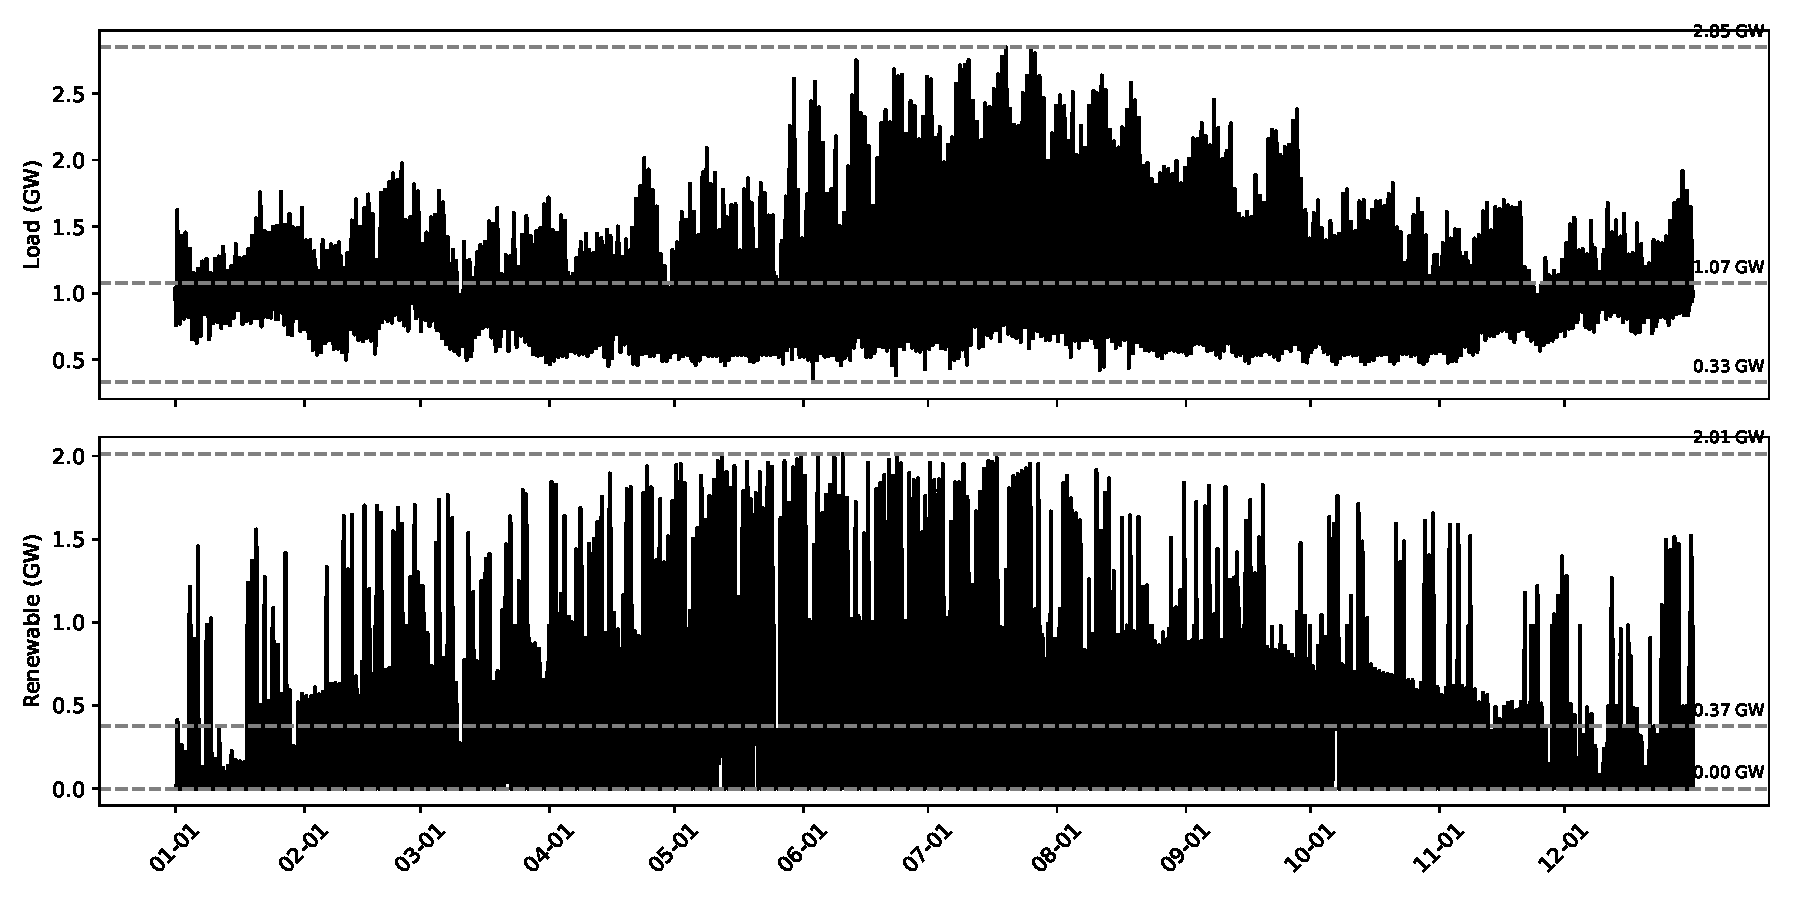
\includegraphics[width=0.8\columnwidth]{./figures/load_renewable.pdf}
\end{figure}

\BIT
\item average load $1.07$ GW, average renewable $0.37$ GW, maximum fossil $1.25$ GW
\item $10\%$ shortfall rate, \ie, \ fraction of time periods we cannot meet load
\EIT
	
\end{frame}

\begin{frame}{Shortfall}
	
\begin{figure}
\centering
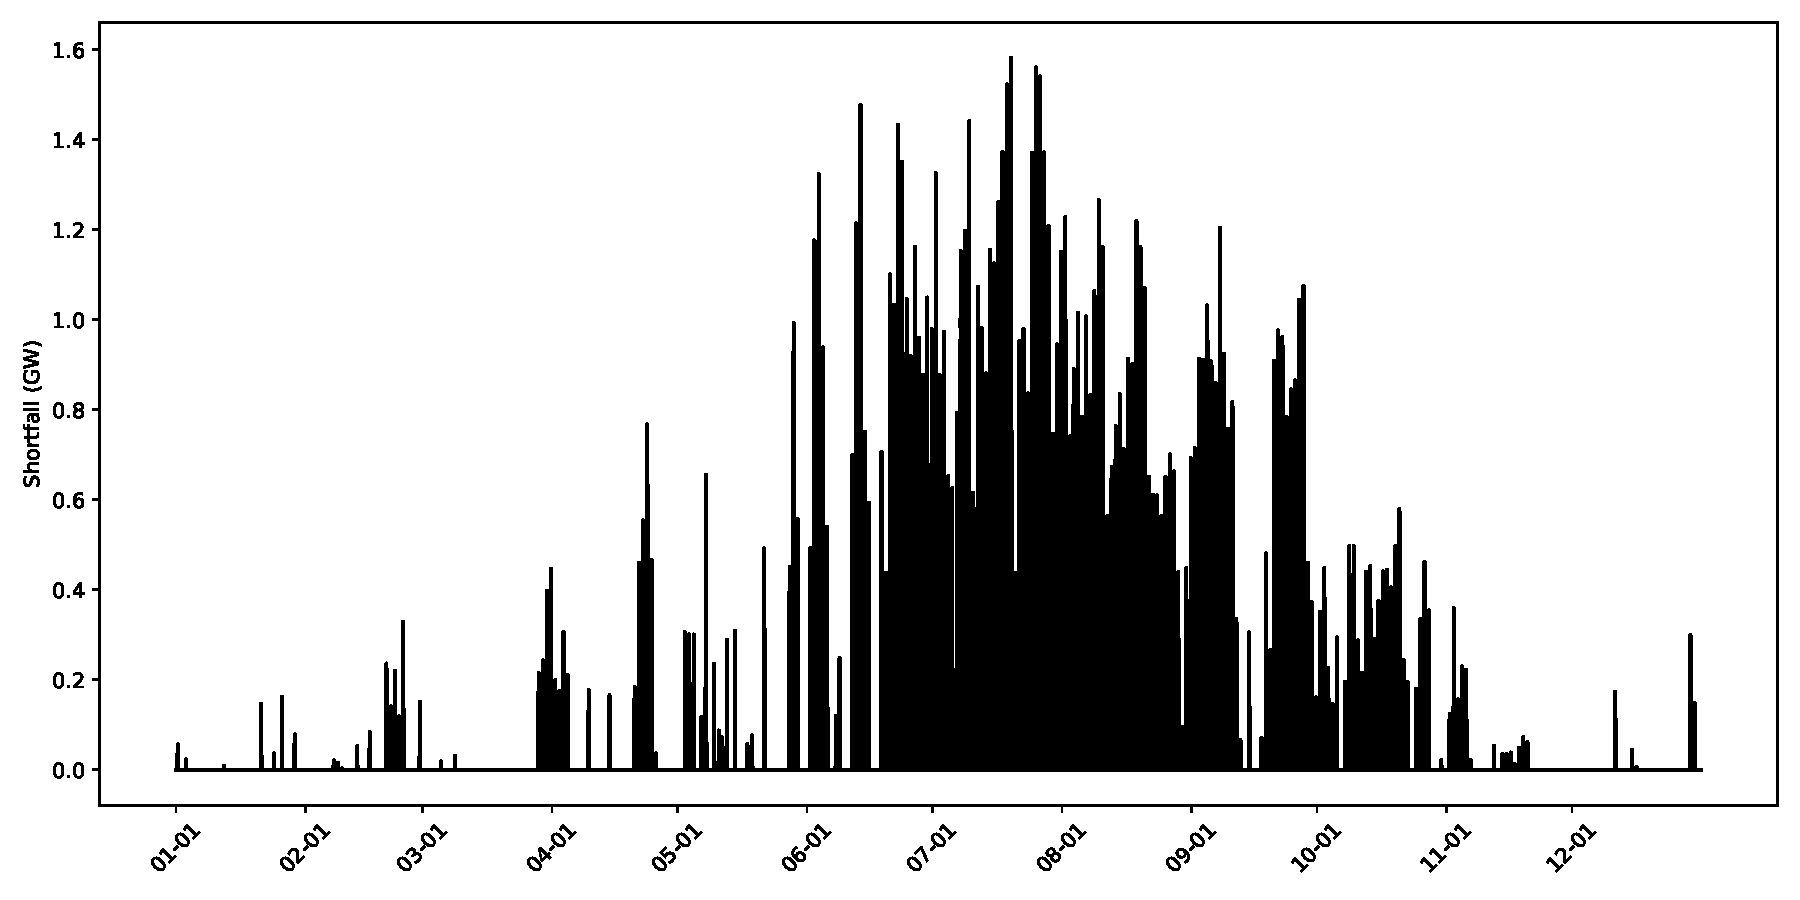
\includegraphics[width=0.8\columnwidth]{./figures/shortfall.pdf}
\end{figure}

\BIT
\item we have enough energy surplus, it just does not come at the right time
\item we will use a battery to move the energy across time
\EIT
\end{frame}

\begin{frame}[fragile]{Model}
    \begin{columns}
        \begin{column}{0.46\textwidth}
    \[
        \begin{array}{ll}
            \mbox{minimize}   &  \frac{1}{T}\sum_{t=1}^{T} \gamma s_t + \alpha u_t + \beta u_t^2 \\
            \mbox{subject to} & q_1 = q_{T+1}, \\
            & q_{t+1} = q_t - b_t, \; t = 1, \ldots, T, \\
            & b + r + u = l-s, \\
            & 0 \leq s \leq l, \\
            & 0 \leq r \leq R, \\
            & 0 \leq q \leq Q \ones, \\
            & 0 \leq u \leq G \ones, \\
        \end{array}
    \]
    $\alpha$, $\beta$, $\gamma$ are hyperparameters
    (we set $\alpha = 1.25$, $\beta = 0.5$, $\gamma = 10$)
    \vfill
    \end{column}
    \begin{column}{0.54\textwidth}
    \vfill
\begin{lstlisting}[language=mypython, basicstyle=\footnotesize\ttfamily, belowskip=0em]
T = R.shape[0]
b = cp.Variable(T)
q = cp.Variable(T+1, nonneg=True)
r = cp.Variable(T, nonneg=True)
u = cp.Variable(T, nonneg=True)
s = cp.Variable(T, nonneg=True)
cons = [q[0] == q[-1],r <= R,
    q <= Q, u <= G, s <= l,
    cp.diff(q) == -b,
    b + r + u == l - s]
obj = 1/T*(10*cp.sum(s) + 1.25*cp.sum(u) 
        + 0.5*cp.sum_squares(u))
prob = cp.Problem(cp.Minimize(obj), cons)
\end{lstlisting}
    \BIT
    \item has $43802$ variables
    \item takes $\approx0.5$ seconds on average
    \EIT
    \end{column}
    \end{columns}
\end{frame}

\begin{frame}{Shortfall vs. storage}
\begin{columns}
    \begin{column}{0.6\textwidth}
        \begin{figure}
            \centering
            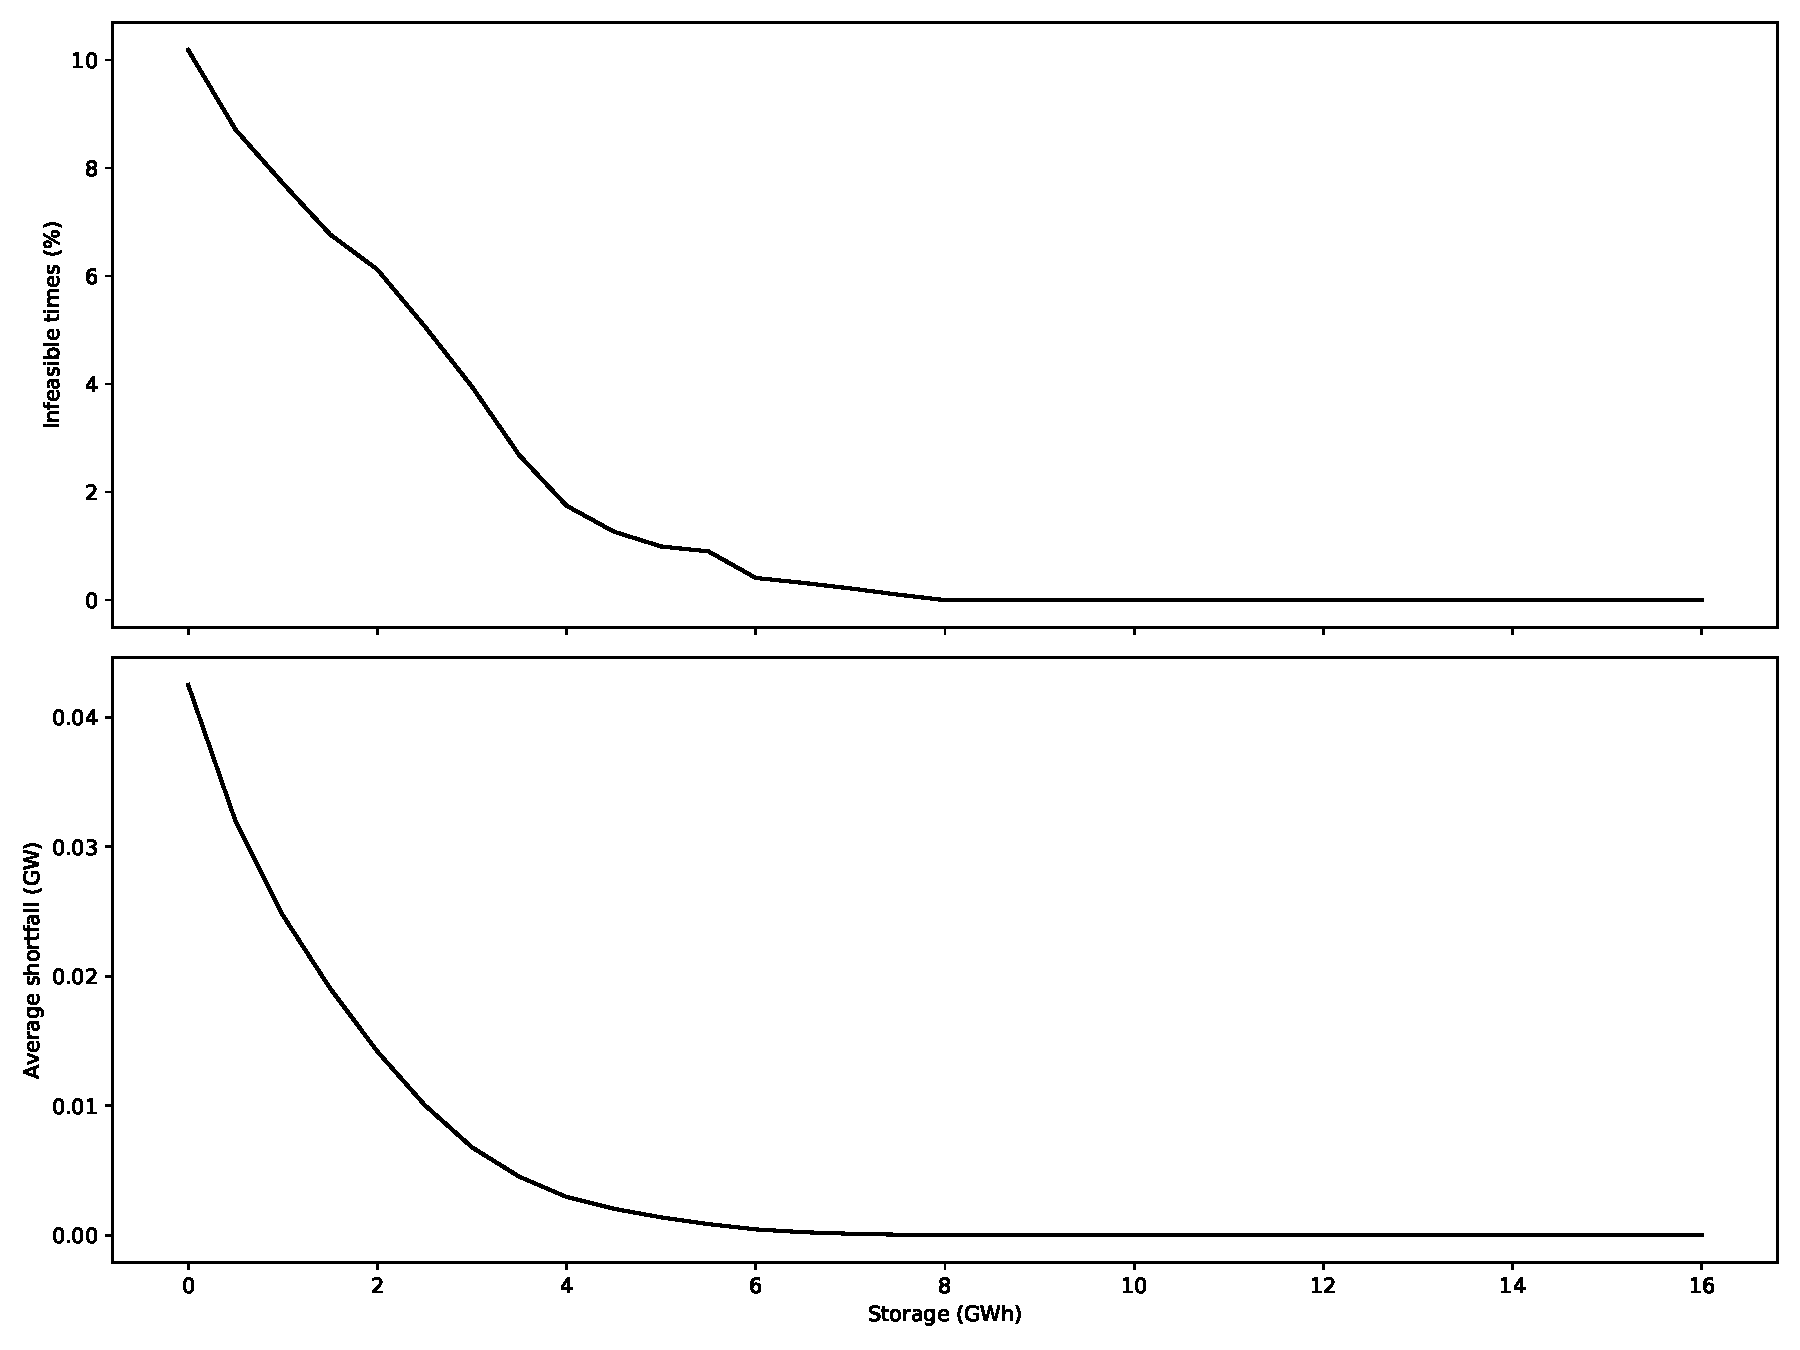
\includegraphics[width=\columnwidth]{./figures/p1.pdf}
        \end{figure}
    \end{column}
    \begin{column}{0.4\textwidth}
        \begin{itemize}
            \item $8$ GWh storage enough to prevent shortfall ($\approx 8$ hours of load)
            \item $3$ GWh enough to reduce infeasible times more than a factor of $2$
        \end{itemize}
    \end{column}
\end{columns}
\end{frame}

\begin{frame}{Fossil vs. storage}
\begin{columns}
    \begin{column}{0.6\textwidth}
        \begin{figure}
            \centering
            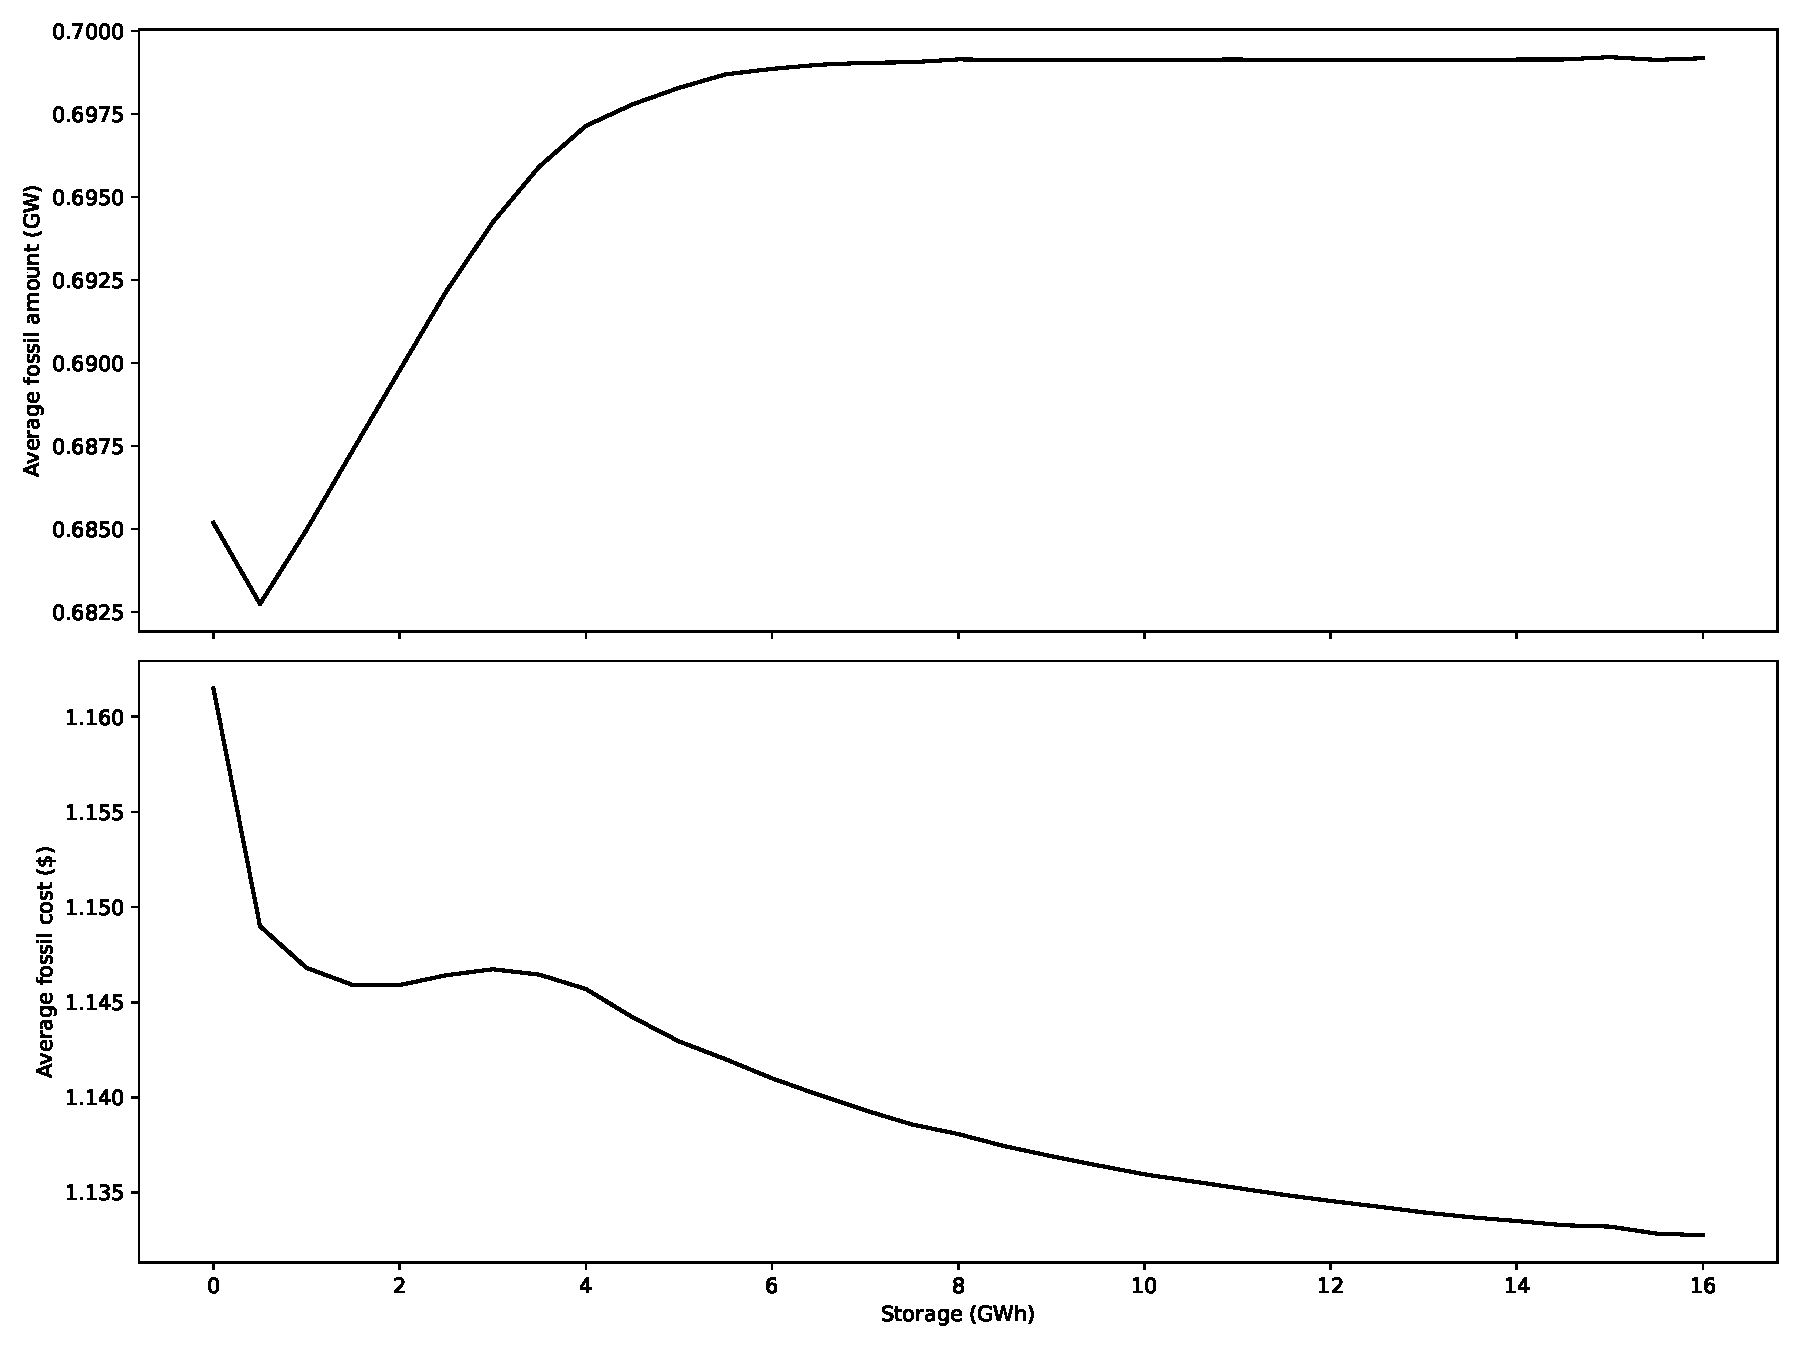
\includegraphics[width=\columnwidth]{./figures/p2.pdf}
        \end{figure}
    \end{column}
    \begin{column}{0.4\textwidth}
        \begin{itemize}
            \item average fossil generation ($\approx 0.7$ GW) does not change much with storage
            \item it is equal to the difference between average load ($1.07$ GW) and renewable ($0.37$ GW)
            \item average fossil cost decreases with storage
        \end{itemize}
    \end{column}
\end{columns}
\end{frame}

\begin{frame}{Renewables vs. storage}
\begin{columns}
    \begin{column}{0.6\textwidth}
        \begin{figure}
            \centering
            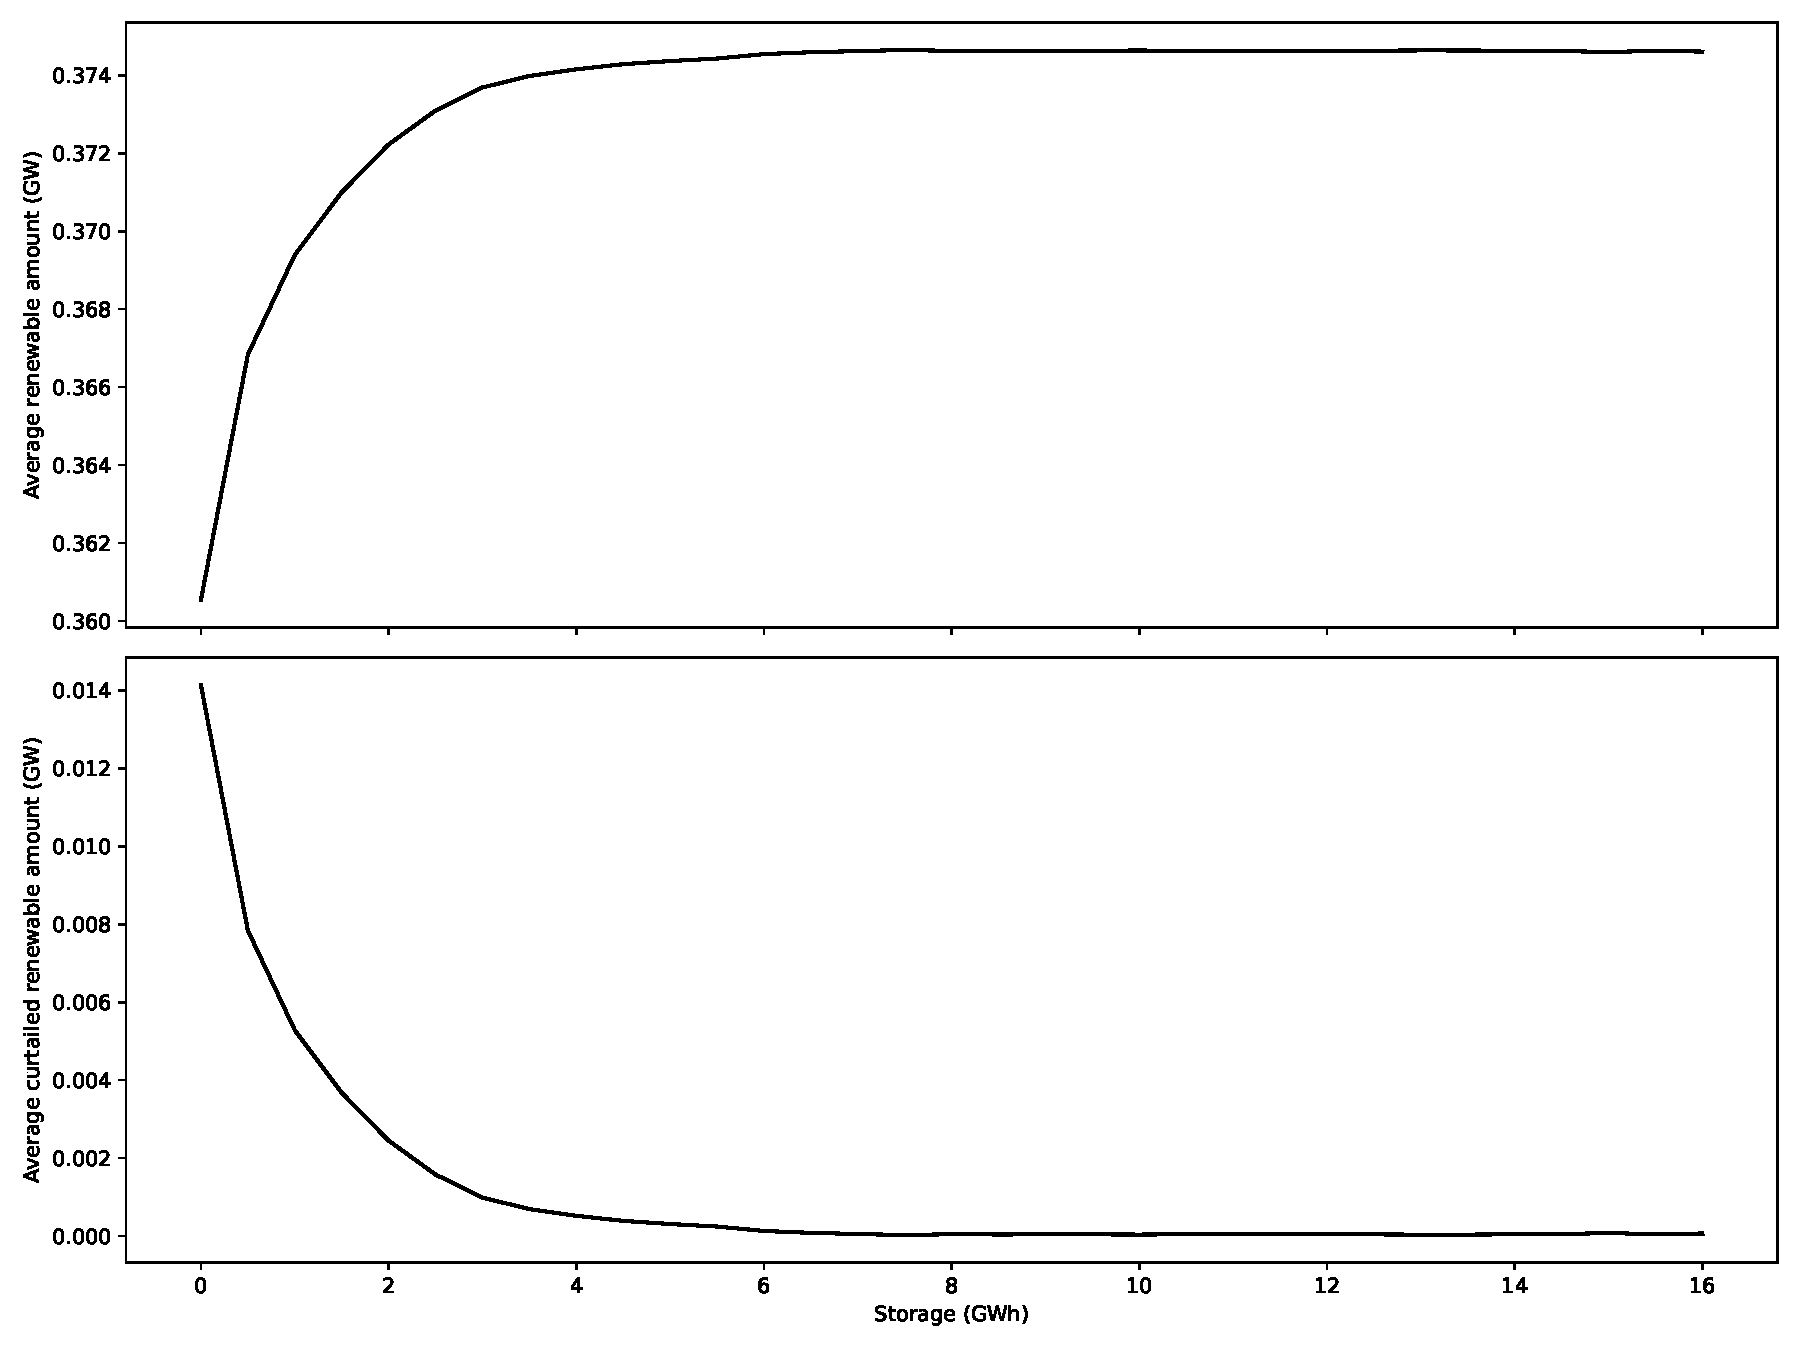
\includegraphics[width=\columnwidth]{./figures/p3.pdf}
        \end{figure}
    \end{column}
    \begin{column}{0.4\textwidth}
        \begin{itemize}
            \item renewable use increases with storage
            \item curtailed renewable decreases with storage
        \end{itemize}
    \end{column}
\end{columns}
\end{frame}

\begin{frame}{Profiles with low and high storage}
\begin{columns}
    \begin{column}{0.5\textwidth}
        \begin{figure}
            \centering
            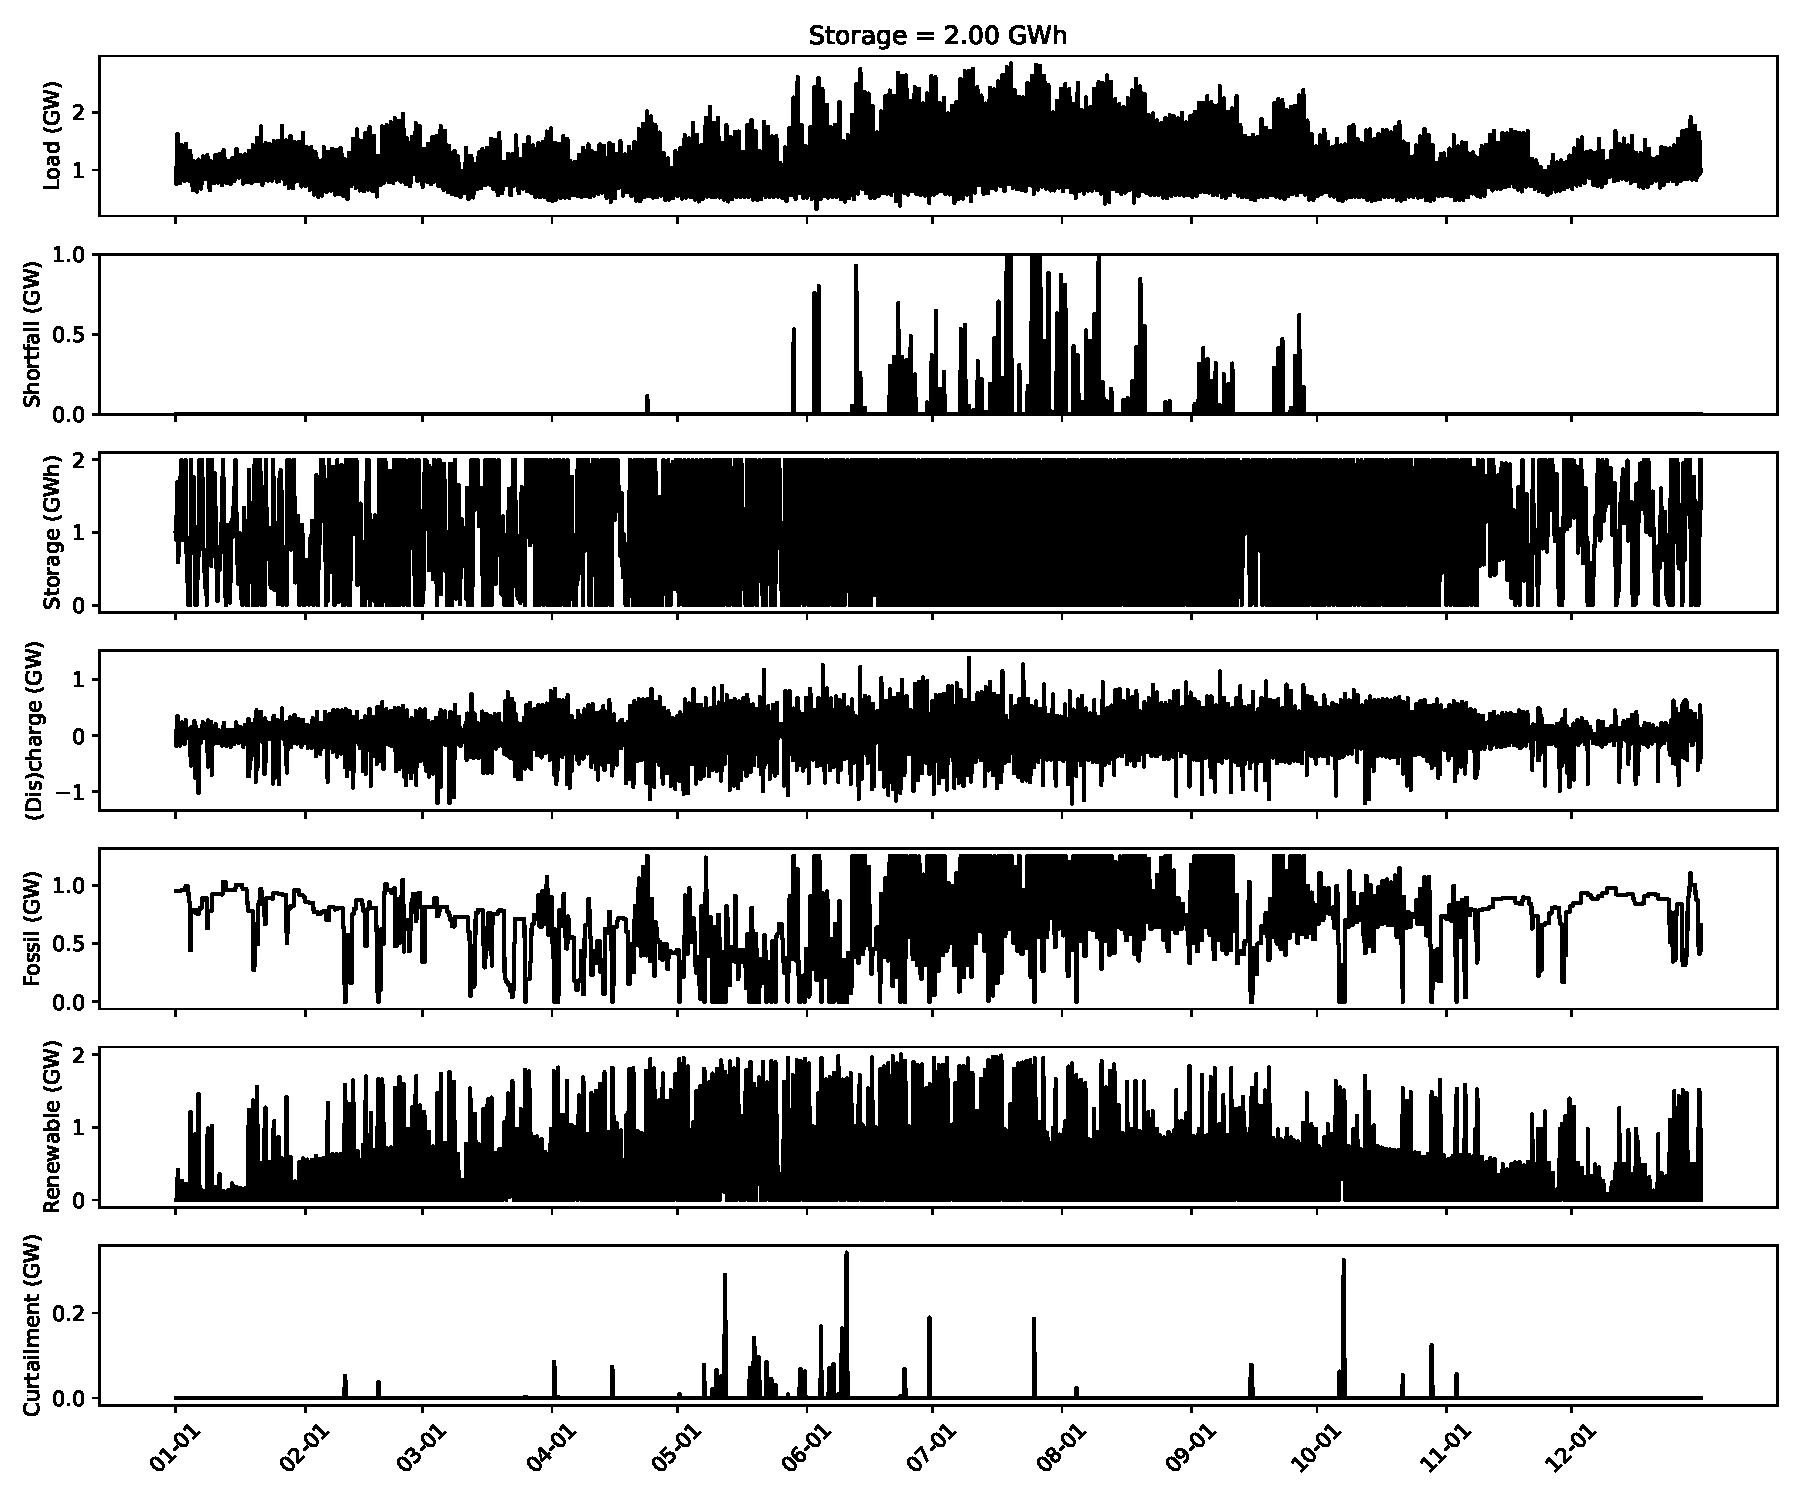
\includegraphics[width=\columnwidth]{./figures/p4.pdf}
        \end{figure}
    \end{column}
    \begin{column}{0.5\textwidth}
        \begin{figure}
            \centering
            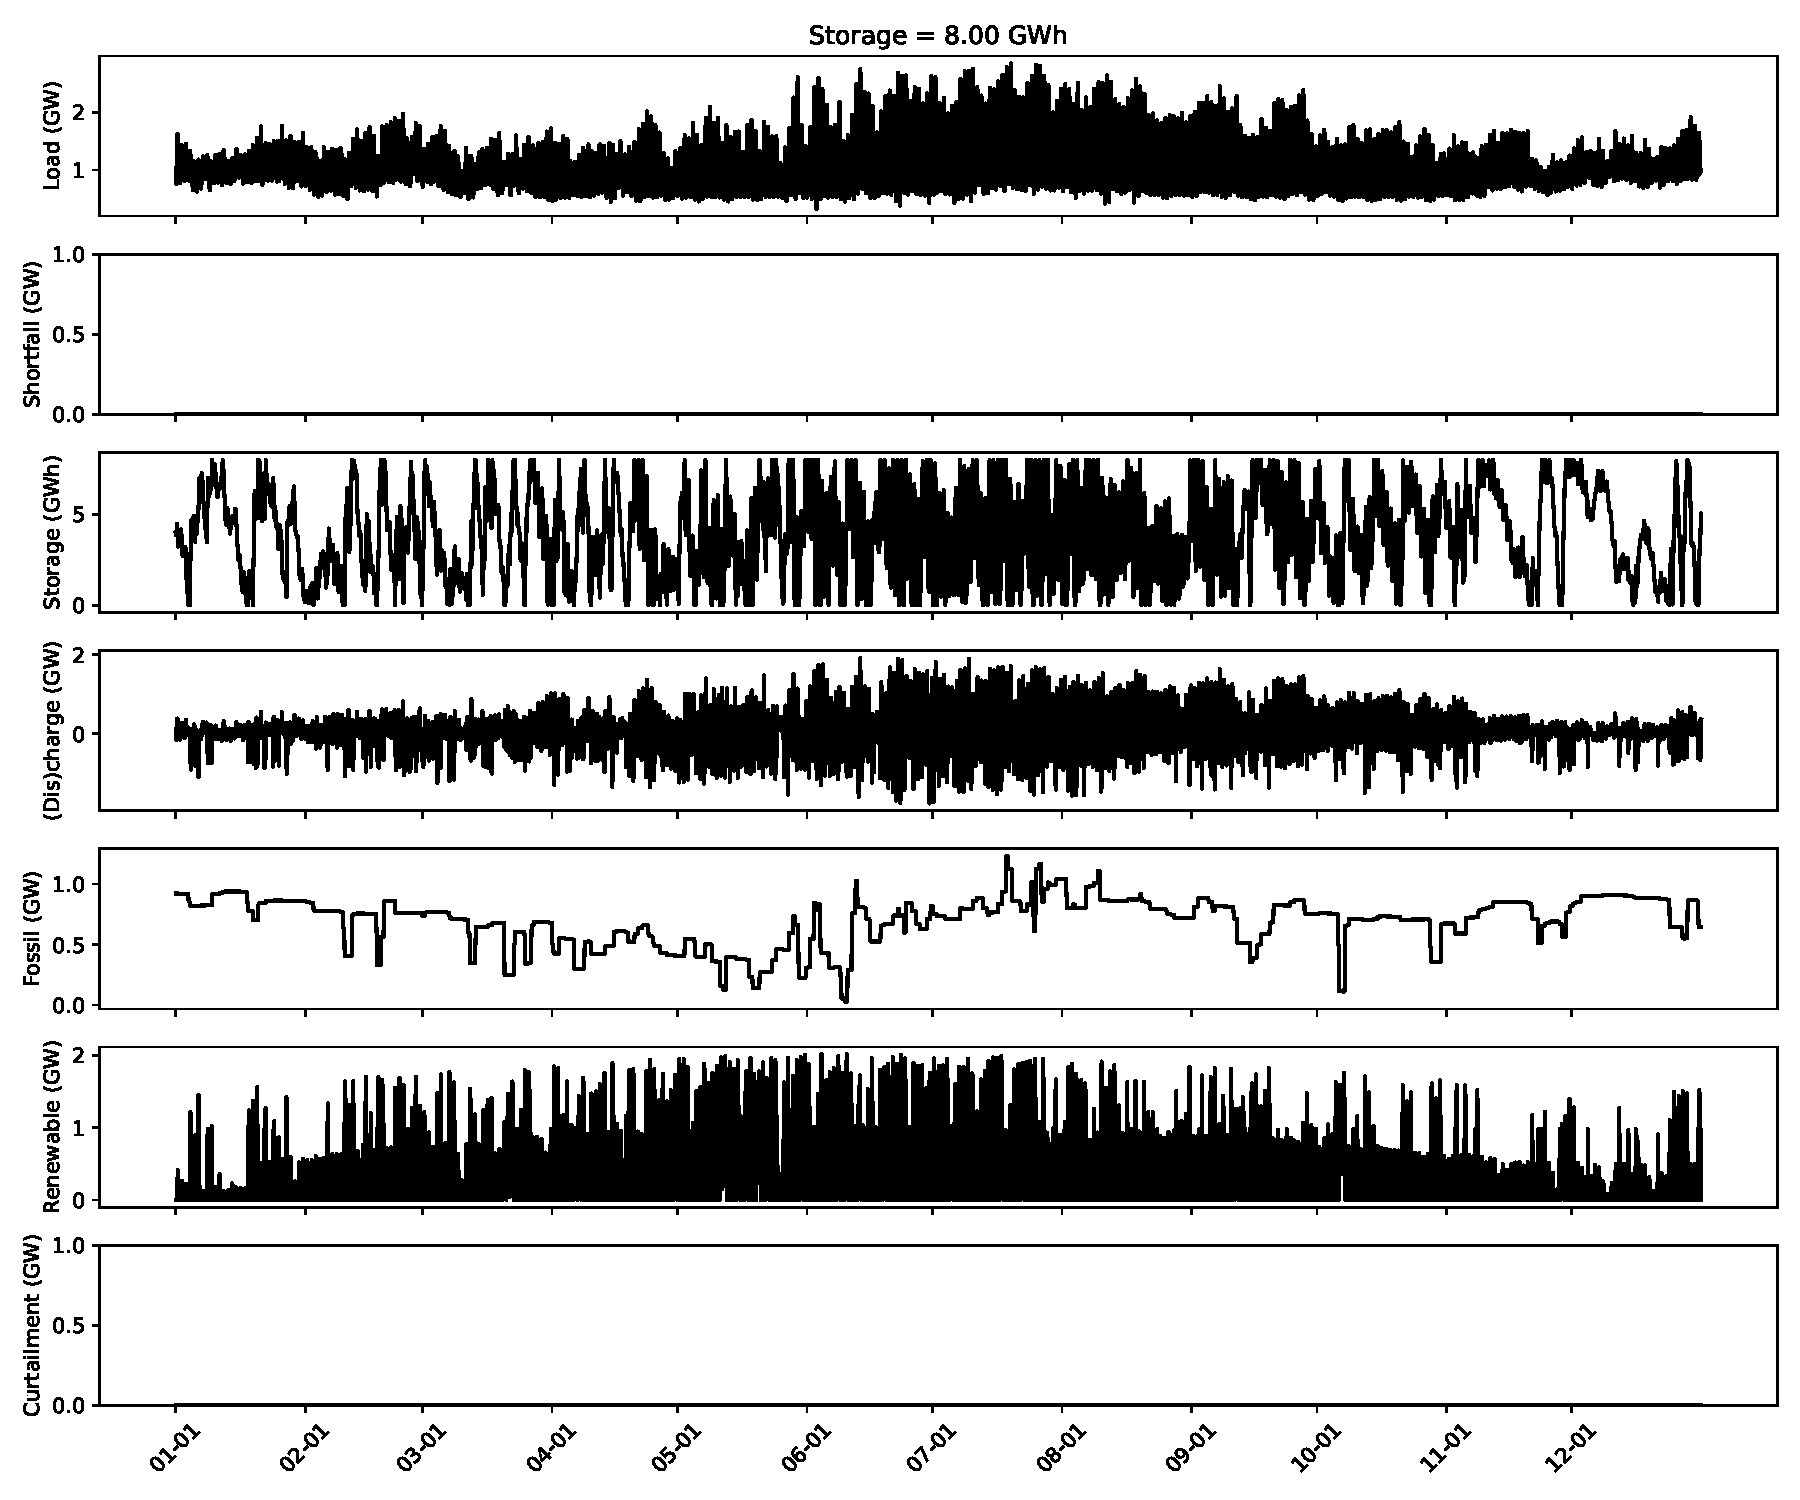
\includegraphics[width=\columnwidth]{./figures/p5.pdf}
        \end{figure}
    \end{column}
\end{columns}
\vfill
\BIT 
\item fossil generation more constant with increased storage
\item increased storage decreases curtailment and prevents shortfall
\EIT
\end{frame}

\begin{frame}{Zooming in for fixed storage}
\begin{columns}
    \begin{column}{0.5\textwidth}
        \begin{figure}
            \centering
            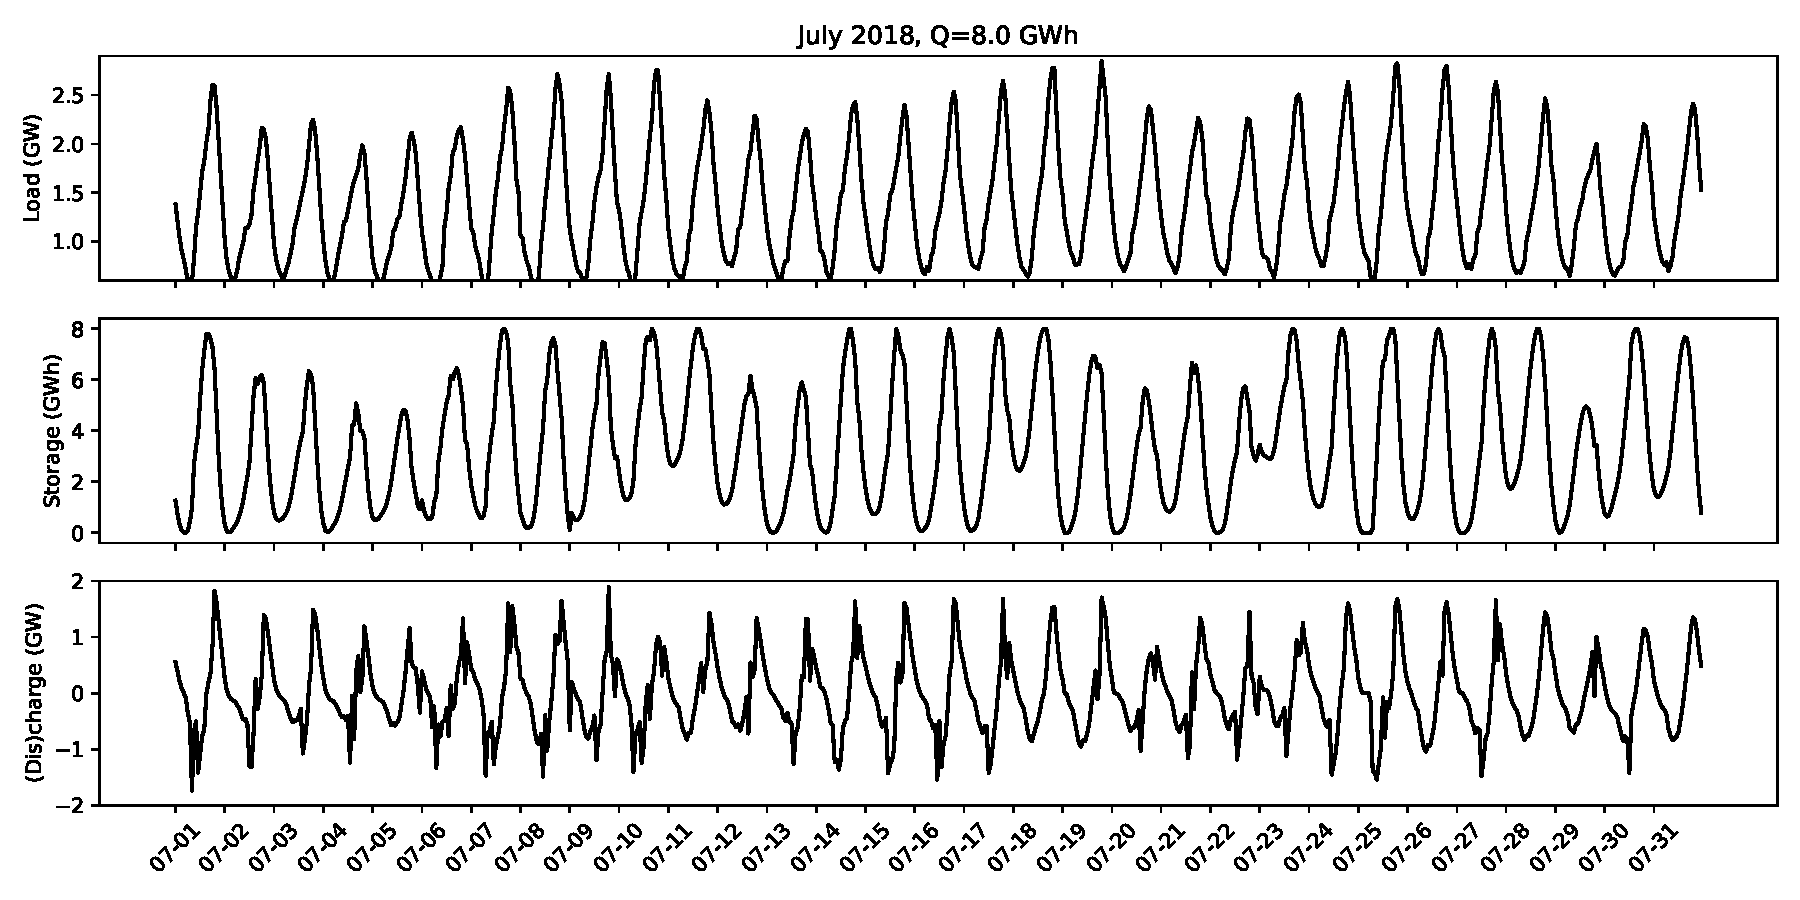
\includegraphics[width=\columnwidth]{./figures/p7.pdf}
        \end{figure}
    \end{column}
    \begin{column}{0.5\textwidth}
        \begin{figure}
            \centering
            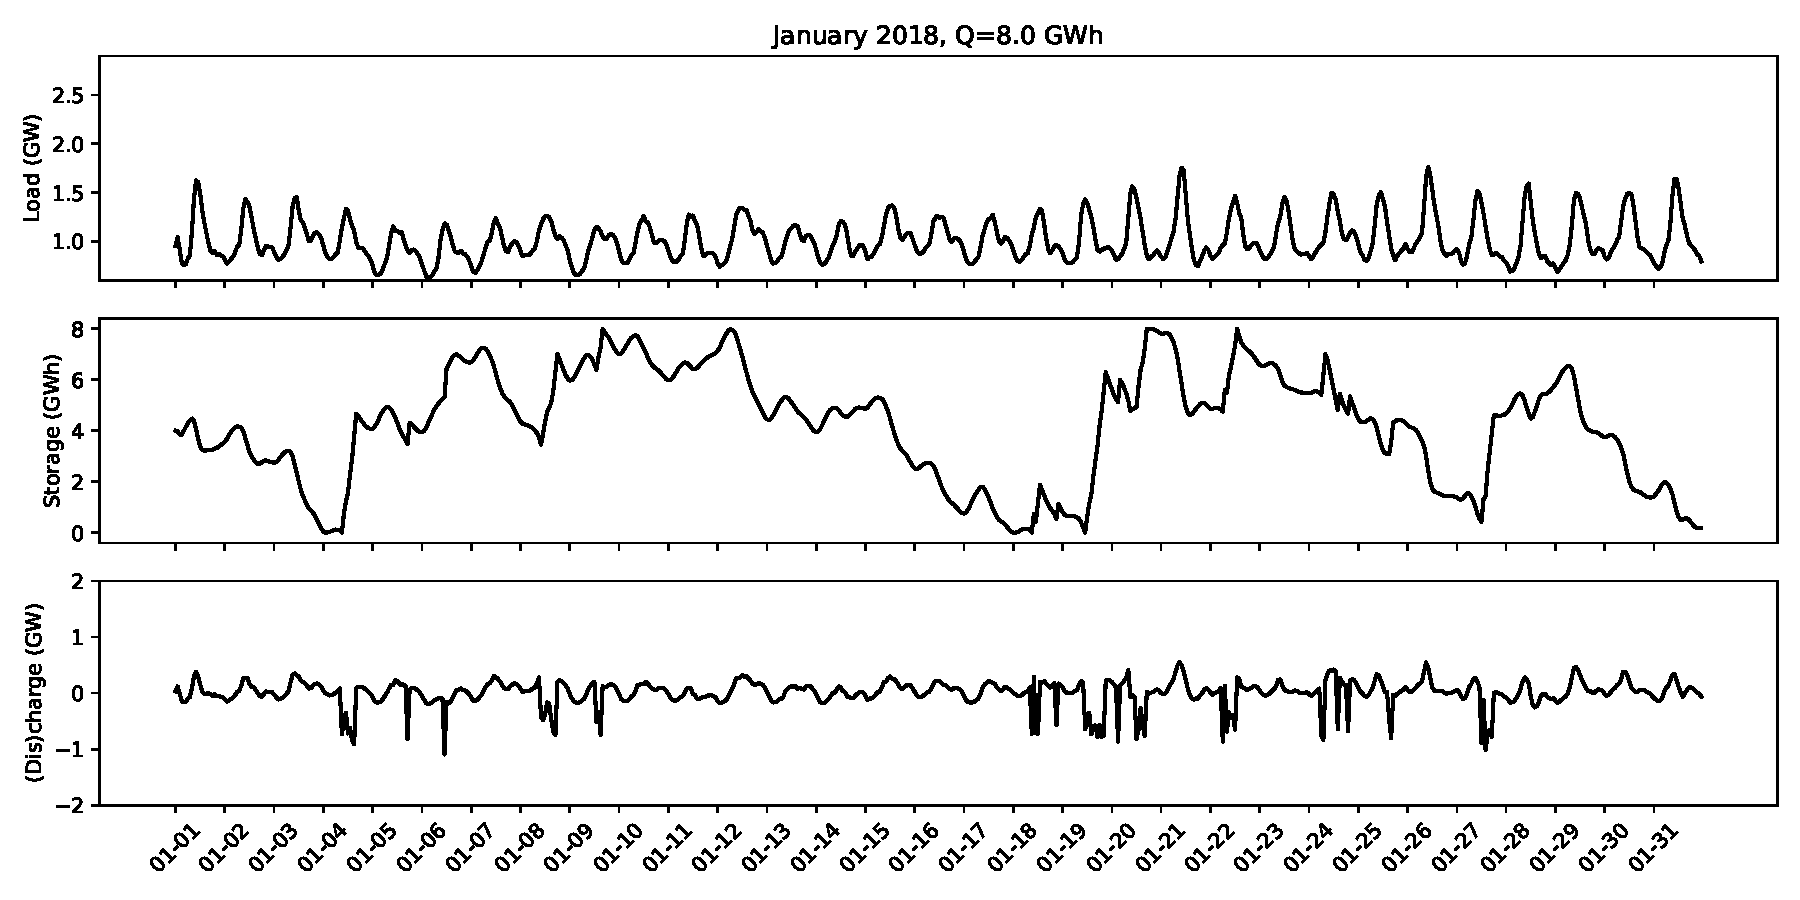
\includegraphics[width=\columnwidth]{./figures/p8.pdf}
        \end{figure}
    \end{column}
\end{columns}
\vfill
\BIT 
\item peak load periods (july) have more volatile storage than off-peak periods (january)
\item high (dis)charge can be detrimental to battery life
\EIT
\end{frame}

\begin{frame}{Next steps} 
\BIT
\item more detailed model (ramp rate on fossil, charge/discharge penalty)
\item model predictive control (MPC)
\item simple and sophisticated forecasters (time-dependent, AR)
\EIT
\end{frame}
    

\begin{frame}{Outreach}
\begin{columns}
    \begin{column}{0.6\textwidth}
        \begin{figure}
            \centering
            
\includegraphics[width=\columnwidth]{./figures/cybercon_program.png}
        \end{figure}
    \end{column}
    \begin{column}{0.4\textwidth}
        \begin{itemize}
            \item participated in 2024 Cybersecurity \& Technology Innovation Conference
            \href{https://www.doecybercon.com/Program/Agenda}{(click to acces the program \& slides)}
            \item abstract accepted to 2024 EU PVPMC
            \href{https://www.sandia.gov/app/uploads/sites/243/dlm_uploads/2024/08/2024-European-PVPMC-Program-V9.pdf}{(click to acces the program)}
            \item currently working on a manuscript
        \end{itemize}
    \end{column}
\end{columns}
\end{frame}
    


	

\end{document}
